% platex report && dvipdfmx report.dvi && open report.pdf
\documentclass{jsarticle}
\usepackage{listings,jlisting}
\usepackage{url}
\usepackage[dvipdfmx]{graphicx}
\usepackage[hang,small,bf]{caption}
\usepackage[subrefformat=parens]{subcaption}
\captionsetup{compatibility=false}
\lstset{
  basicstyle={\ttfamily},
  identifierstyle={\small},
  commentstyle={\smallitshape},
  keywordstyle={\small\bfseries},
  ndkeywordstyle={\small},
  stringstyle={\small\ttfamily},
  frame={tb},
  breaklines=true,
  columns=[l]{fullflexible},
  numbers=left,
  xrightmargin=0zw,
  xleftmargin=3zw,
  numberstyle={\scriptsize},
  stepnumber=1,
  numbersep=1zw,
  lineskip=-0.5ex
}

\begin{document}

\title{情報システム論実習 テキスト分析演習課題 07月09日分}
\author{6930318812 沖野 雄哉}
\maketitle

\section{利用した表現手法}
ベクトルベースの手法の中からBoWとtf-idfを用いて表現した。

\section{利用した距離尺度}
以下の二つの距離尺度を利用した。
\begin{itemize}
  \item ユークリッド距離
  \item コサイン類似度
\end{itemize}

\section{入力ドキュメント}
以下の文書を対象に分析を行った。

\begin{itemize}
  \item View update is an important mechanism that allows updates on a view by translating them into the corresponding updates on the base relations.
  \item The existing literature has shown the ambiguity of translating view updates.
  \item To address this ambiguity, we propose a robust language-based approach for making view update strategies programmable and validatable.
  \item Specifically, we introduce a novel approach to use Datalog to describe these update strategies.
  \item We present a fragment of the Datalog language for which our validation is both sound and complete.
  \item We propose a validation algorithm to check the well-behavedness of the written Datalog programs.
  \item This fragment not only has good properties in theory but is also useful for solving practical view updates.
  \item Furthermore, we develop an algorithm for optimizing user-written programs to efficiently implement updatable views in relational database management systems.
  \item We have implemented our proposed approach.
  \item The experimental results show that our framework is feasible and efficient in practice.
\end{itemize}

\section{実行結果}
ドキュメント同士の距離を計算し、ヒートマップで表現した結果次のようになった。

\begin{figure}[h]
 \begin{minipage}[b]{0.50\linewidth}
  \centering
  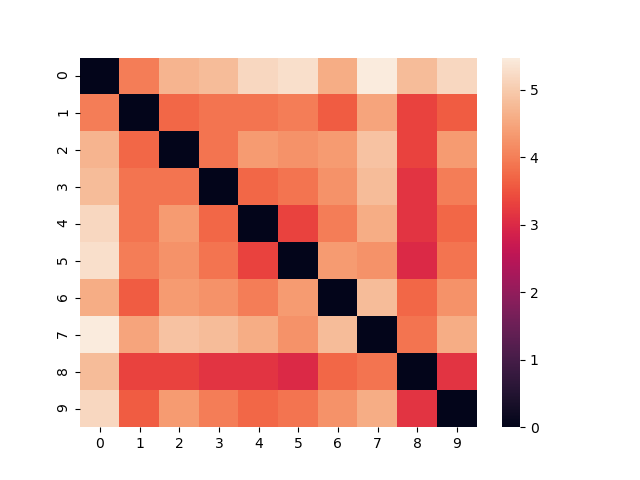
\includegraphics[keepaspectratio, scale=0.42]
  {./euclidean_distance_bows.png}
  \subcaption{BoW, ユークリッド距離}\label{euclidean_bow}
 \end{minipage}
 \begin{minipage}[b]{0.50\linewidth}
  \centering
  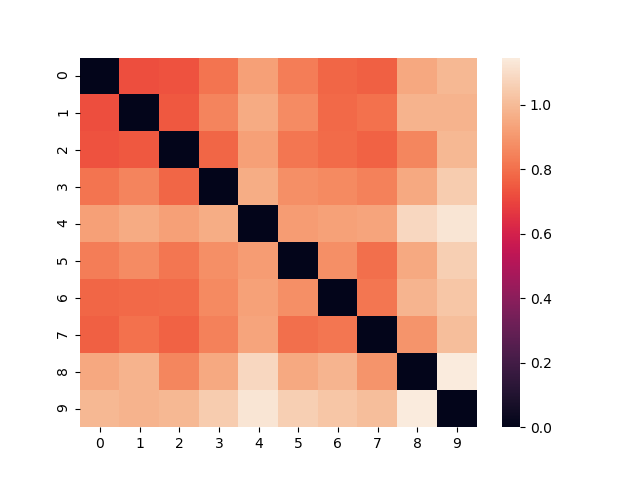
\includegraphics[keepaspectratio, scale=0.42]
  {./euclidean_distance_tfidfs.png}
  \subcaption{tf-idf, ユークリッド距離}\label{euclidean_tfidf}
 \end{minipage}
 \begin{minipage}[b]{0.50\linewidth}
  \centering
  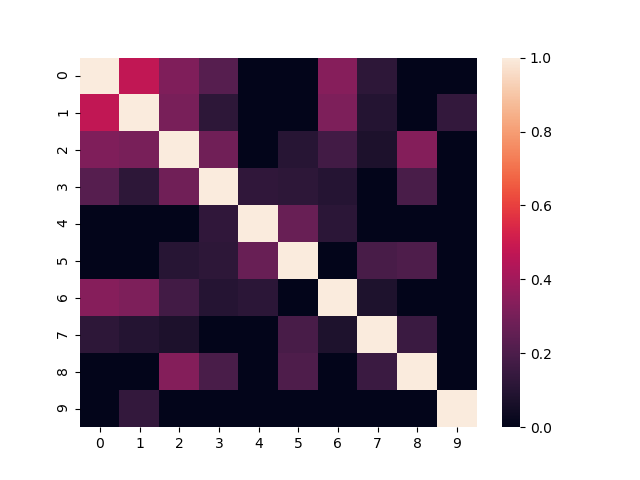
\includegraphics[keepaspectratio, scale=0.42]
  {./cosine_similarity_bows.png}
  \subcaption{BoW, コサイン類似度}\label{cosine_bow}
 \end{minipage}
 \begin{minipage}[b]{0.50\linewidth}
  \centering
  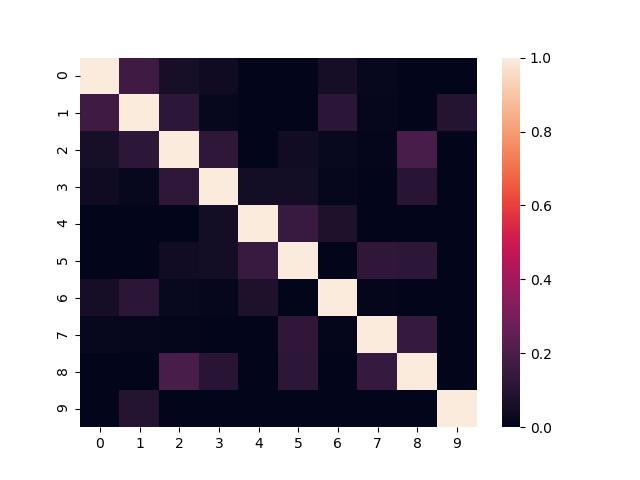
\includegraphics[keepaspectratio, scale=0.42]
  {./cosine_similarity_tfidfs.png}
  \subcaption{tf-idf, コサイン類似度}\label{cosine_tfidf}
 \end{minipage}
\end{figure}

\section{実行結果の考察}

コサイン類似度は大きな違いはないが、全体的に類似度が下がっていると捉えられる。
これは、類似度が大きい二つの文書は同じ語をドキュメントに含んでいるため、tfidfでの表現はベクトルのノルムが小さくなり、コサイン類似度が小さくなったと考えられる。\\
また、ユークリッド距離については、全体的な傾向として距離関係が逆転しているように見えた。
文書9、10に着目して、それぞれのtfidfの値を出力した結果が以下の図である。
文書9は文書が小さく3語しかないため、全体的にtfの値が大きくなり、tf-idfの値が大きくなっている。
また文書10は文書10にしか含まれない単語を多く含んでいるが、語数が多いため、tf-idf値が小さくなっている。
BoWにおけるユークリッド距離は単語数が少ない文書については小さくなる傾向があるが、上記の理由からtf-idfで表現した場合は単語数が少ない文書の方がユークリッド距離が大きくなり、距離関係の逆転が起こっているのではないかと考えられる。

\section{感想}
文書を単語の集合として表現することでおおまかに文書の類似度を測ることができると分かった。
直感的には時系列的な情報が全てなくなっている状態でも大丈夫なのか気になる。
文書表現に時系列情報を含める手法があるのか、その場合だとどのように変わるのか知りたい。
ただ時系列を考慮すると、大量のデータを処理して類似する文書を取得したいケースなどを考えると、計算量の問題がありそうだとも思うので一長一短あるとも思う。
また文書の類似度をヒューリスティックにでも評価することは難しいと感じたので、どのような評価指標が用いられているのか調べたい。

\section{ソースコード}
\url{https://github.com/oky-123/soc_info_mining}

\begin{figure}[h]
 \begin{minipage}[b]{0.50\linewidth}
  \centering
  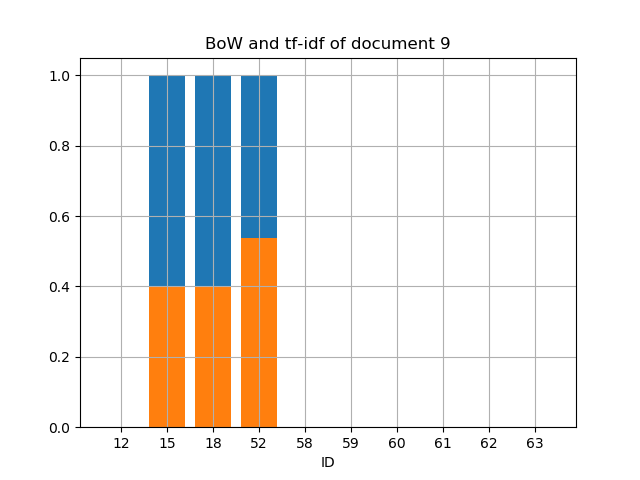
\includegraphics[keepaspectratio, scale=0.42]
  {./doc_8.png}
  \subcaption{blue: BoW, orange: tf-idf}\label{doc_8}
 \end{minipage}
 \begin{minipage}[b]{0.50\linewidth}
  \centering
  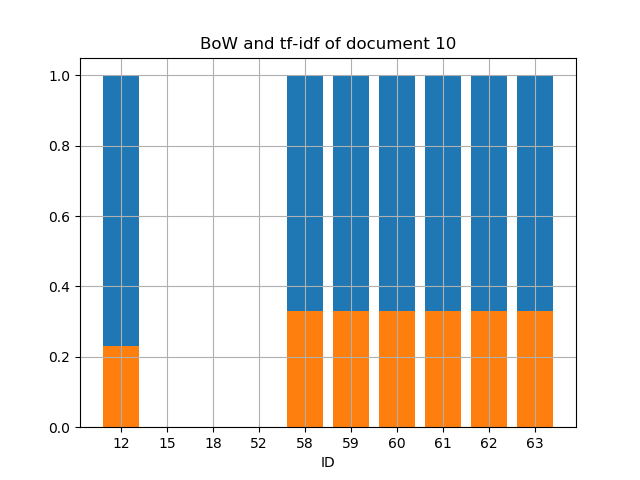
\includegraphics[keepaspectratio, scale=0.42]
  {./doc_9.png}
  \subcaption{blue: BoW, orange: tf-idf}\label{doc_9}
 \end{minipage}
\end{figure}


\end{document}
